\chapter{Experimentální uspořádání}

\subsection{Optické měřící přístroje}

\subsubsection{Bruker VERTEX 80v}
Jedná se o je vakuový FTIR spektrofotometr, který obsahuje Michelsonův interferometr, se zrcadlem kmitajícím na vzduchovém polštáři. Během všech měření byl používán speciální nástavec, díky němuž bylo možné provádět správné absolutní měření propustnosti. V průběhu měření jsou vzorky umístěny svisle na držáku v měřící komoře, ve které je po dobu měření udržováno vakuum 2,51\,hPa, což slouží k minimalizace vlivu okolního prostředí a vlhkosti na průběh měření. Výrobcem udávaní spektrání rozlišení spektrometru je minimálně 0,2\,cm$^{-1}$ při běžných laboratorních podmínkách. Spektrální rozsah spektrofotometru je 1333 -- 27000\,cm$^{-1}$, ale při požití vhodných rozšíření je možné měřit i do FIR a UV/VIS oblastí \cite{vertex}.

FIXME: Vyfotit obrázek.

%\begin{figure}
%  \centering
%  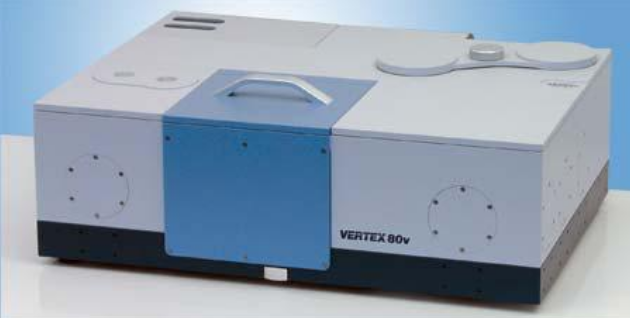
\includegraphics[width=120mm]{vertex80v.png}
%  \caption{Spektrofotometr Bruker VERTEX 80v.}
%  \label{verteximg}
%\end{figure}

\subsubsection{LAMBDA 1050 UV/Vis/NIR}
LAMBDA 1050 UV/Vis/NIR od firmy PerkinElmer je dvoukanálový spektrofotometr. Jako zdroj slouží halogen-rtuťová a deuteriová lampa.  Přístroj obsahuje dva monochromátory (holografické difrakční mřížky s 1440 proužky,vrypy? na milimetr pro UV/Vis oblast a s 360 proužky na milimetr pro IR oblast)  (FIXME: holographic grating monochromator with 1440 lines/mm UV/Vis blazed at 240 nm and 360 lines/mm NIR blazed at 1100 nm,). Pro dělení svazku na dva kanály je použit chopper. Udávaný spektrální rozsah je 175--3300\,nm, nicméně pro měření pod 185\,nm je potřeba chlazení dusíkem. Použitý detektor pro viditelnou a UV oblast je fotonásobič R6872. Pro oblast 860--1800\,nm je použit InGaAs detektor, chlazený peltierovým článkem a pro oblast 1800--2500\,nm PbS detektor, taktéž chlazený peltierovým článkem. Spektrální rozlišení výrobce udává jako minimálně 0,05\,nm. Přístroj obsahuje optickou kompenzaci pro různé tloušťky vzorků \cite{lambda}.

FIXME: Vyfotit obrázek.

%\begin{figure}
%  \centering
%  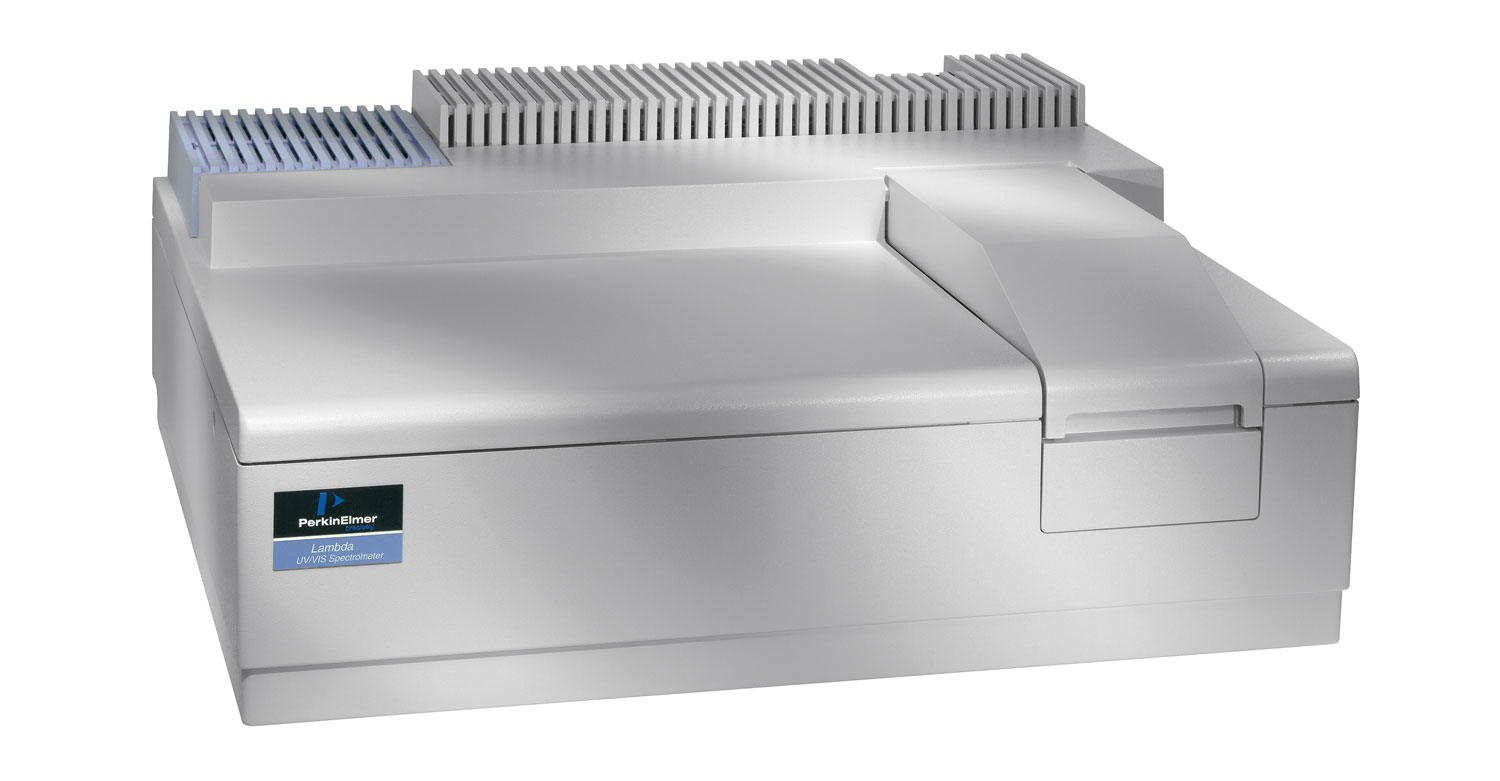
\includegraphics[width=120mm]{LAMBDA.jpg}
%  \caption{Spektrofotometr LAMBDA 45 UV/Vis.}
%  \label{lambdaimg}
%\end{figure}

\subsubsection{Jobin-Yvon UVISEL}
Schéma elipsometru Jobin-Yvon UVISEL je znázorněno na schématu \ref{fig:elipsometrimg} (FIXME: udělat schéma v inkscapu). Udávaný spektrální rozsah tohoto přístroje je od 190\,nm do 2000\,nm. Hlavy elipsometru jsou umístěny na goniometru, z toho důvodu může být měření prováděno pod různými úhly. Běžně se měří úhly dopadu 55$^\circ$, 60$^\circ$, 65$^\circ$, 70$^\circ$ a 75$^\circ$. Jedná se o fázově modulovaný elipsometr. Měření probíhá tak, že z lampy L vychází chromatické nepolarizované světlo, které poté prochází přes polarizátor P. Tam dojde k jeho lineární polarizaci, odráží se od vzorku a přes kompenzátor C, analyzátor A a monochromátor dopadá na detektor D.

FIXME: Taky možná fotku?

%\begin{figure}
%  \centering
%  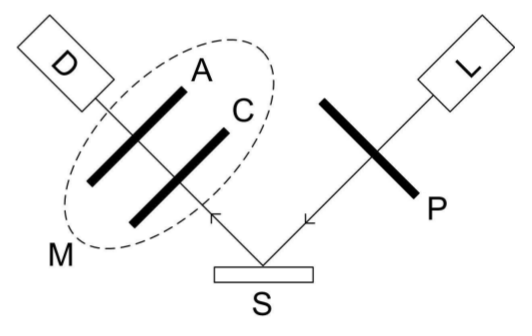
\includegraphics[width=120mm]{schema-elipsometru.png}
%  \caption{Schéma elipsometru UVISEL (P--polarizátor, C--kompenzátor, D--detektor, L--lampa, M--modulátor, A--analyzátor, S--substrát), obrázek převzat z \cite{fialova2009}.}
%  \label{fig:elipsometrimg}
%\end{figure}

\cleardoublepage
